\documentclass{beamer}
\usepackage{amsmath}
\usepackage{amssymb}
\usepackage{amsfonts}
\usepackage[utf8]{inputenc}
\usepackage{graphics}
\usepackage{hyperref}
\usepackage{xcolor}
\usepackage{wasysym}
\usepackage{listings}
\usepackage{tikz}
\usepackage[normalem]{ulem}
\usepackage{textcomp}
\usepackage{verbatim}
\usepackage[T1]{fontenc}
\usepackage{lmodern}
\usepackage[framemethod=tikz]{mdframed}
\usetikzlibrary{shapes.callouts,shadows, calc}

\tikzset{note/.style={rectangle callout, rounded corners,fill=gray!20,drop shadow,font=\footnotesize}}    
\newcommand{\tikzmark}[1]{\tikz[overlay,remember picture] \node (#1) {};}    

\newcounter{image}
\setcounter{image}{1}

\makeatletter
\newenvironment{btHighlight}[1][]
{\begingroup\tikzset{bt@Highlight@par/.style={#1}}\begin{lrbox}{\@tempboxa}}
{\end{lrbox}\bt@HL@box[bt@Highlight@par]{\@tempboxa}\endgroup}

\newcommand\btHL[1][]{%
  \begin{btHighlight}[#1]\bgroup\aftergroup\bt@HL@endenv%
}
\def\bt@HL@endenv{%
  \end{btHighlight}%   
  \egroup
}
\newcommand{\bt@HL@box}[2][]{%
  \tikz[#1]{%
    \pgfpathrectangle{\pgfpoint{0pt}{0pt}}{\pgfpoint{\wd #2}{\ht #2}}%
    \pgfusepath{use as bounding box}%
    \node[anchor=base west,rounded corners, fill=green!30,outer sep=0pt,inner xsep=0.2em, inner ysep=0.1em,  #1](a\theimage){\usebox{#2}};
  }%
 \stepcounter{image}
}
\makeatother

\usetheme{Warsaw}
\usecolortheme{lily}
\setbeamercovered{transparent}
\setbeamertemplate{headline}{
  \begin{beamercolorbox}{section in head/foot}
    \vskip2pt\insertnavigation{\paperwidth}\vskip2pt
  \end{beamercolorbox}
}

\setbeamertemplate{footline}{
}

\author{
  {\tiny Tony Morris\\}
}

\xdefinecolor{darkgreen}{rgb}{0,0.35,0}
\lstset{
  tabsize=2,
  basicstyle=\ttfamily,
  moredelim=**[is][\btHL]{`}{`}
}
\lstdefinelanguage{java}{
  morekeywords={abstract,assert,boolean,break%
    byte,case,catch,char,class,const,continue%
    default,do,double,else,enum,extends,false%
    final,finally,float,for,goto,if,implements%
    import,instanceof,int,interface,long,native%
    new,null,package,private,protected,public%
    return,short,static,strictfp,super,switch%
    synchronized,this,throw,throws,transient%
    true,try,void,volatile,while},
  otherkeywords={=,=>,<-,<\%,<:,>:,\#,@},
  sensitive=true,
  morecomment=[l]{//},
  morecomment=[n]{/*}{*/},
  morestring=[b]",
  morestring=[b]',
  morestring=[b]"""
}
\lstdefinelanguage{haskell}{
  morekeywords={class,instance,where,do,data,newtype,default,deriving,module},
  otherkeywords={<-},
  sensitive=true,
  morecomment=[l]{--},
  morecomment=[n]{\{-}{-\}}, 
  morestring=[b]",
  morestring=[b]',
  morestring=[b]"""
}
\lstdefinelanguage{python}{
 keywords={catch, def, float, lambda, in, int, null, self, str, switch, typeof},
 keywordstyle=\color{ForestGreen}\bfseries,
 ndkeywords={boolean, throw, import},
 ndkeywords={return, class, if ,elif, endif, while, do, else, True, False , catch, def},
 ndkeywordstyle=\color{red}\bfseries,
 identifierstyle=\color{black},
 sensitive=false,
 comment=[l]{\#},
 morecomment=[s]{/*}{*/},
 commentstyle=\color{purple}\ttfamily,
 stringstyle=\color{red}\ttfamily,
}
\lstdefinelanguage{scala}{
  morekeywords={abstract,case,catch,class,def,%
    do,else,extends,false,final,finally,%
    for,forSome,if,implicit,import,lazy,match,%
    new,null,object,override,package,%
    private,protected,requires,return,sealed,%
    super,this,throw,trait,true,try,%
    type,val,var,while,with,yield},
  otherkeywords={=,=>,<-,<\%,<:,>:,\#,@},
  sensitive=true,
  morecomment=[l]{//},
  morecomment=[n]{/*}{*/},
  morestring=[b]",
  morestring=[b]',
  morestring=[b]"""
}
\lstdefinestyle{haskell}{
  language=haskell,
  basicstyle=\footnotesize\ttfamily,
  stringstyle=\color{darkgreen}\ttfamily,
  commentstyle=\color{gray}\ttfamily,
  keywordstyle=\footnotesize\color{blue}\ttfamily,
  tabsize=2,
  moredelim=**[is][\btHL]{`}{`}
}
\lstdefinestyle{java}{
  language=java,
  basicstyle=\footnotesize\ttfamily,
  stringstyle=\color{darkgreen}\ttfamily,
  commentstyle=\color{gray}\ttfamily,
  keywordstyle=\footnotesize\color{blue}\ttfamily,
  tabsize=2,
  moredelim=**[is][\btHL]{`}{`}
}
\lstdefinestyle{python}{
  language=python,
  basicstyle=\footnotesize\ttfamily,
  stringstyle=\color{darkgreen}\ttfamily,
  commentstyle=\color{gray}\ttfamily,
  keywordstyle=\footnotesize\color{blue}\ttfamily,
  tabsize=2,
  moredelim=**[is][\btHL]{`}{`}
}
\lstdefinestyle{scala}{
  language=scala,
  basicstyle=\footnotesize\ttfamily,
  stringstyle=\color{darkgreen}\ttfamily,
  commentstyle=\color{gray}\ttfamily,
  keywordstyle=\footnotesize\color{blue}\ttfamily,
  tabsize=2,
  moredelim=**[is][\btHL]{`}{`}
}
% #866eaa
\definecolor{nicta-purple}{rgb}{0.5234,0.4297,0.6640}

\defbeamertemplate*{title page}{customized}[1][] {
  \centering
  \color{nicta-purple}
  \usebeamerfont{title}\inserttitle\par
  \bigskip
  \usebeamerfont{subtitle}\insertsubtitle\par
  \bigskip
  \bigskip
  \bigskip
  \bigskip
  \usebeamerfont{institute}\insertinstitute\par
  \bigskip
  \usebeamerfont{author}\insertauthor\par
  % \usebeamerfont{date}\insertdate\par
  \usebeamercolor[fg]{titlegraphic}\inserttitlegraphic
}

\logo{
\includegraphics[height=0.8cm]{image/nicta.jpg}}


\setbeamercovered{transparent}

\begin{document}

\newmdenv[tikzsetting={draw=black,fill=white,fill opacity=0.7, line width=4pt},backgroundcolor=none,leftmargin=0,rightmargin=0,innertopmargin=4pt]{Conference}

\newmdenv[tikzsetting={draw=black,fill=white,fill opacity=0.7, line width=4pt},backgroundcolor=none,leftmargin=0,rightmargin=0,innertopmargin=4pt,skipbelow=\baselineskip,%
skipabove=\baselineskip]{TitleBox}

\title{\large Perhaps There Is A \tiny{much }\normalsize Better Way}
\institute[NICTA]{National ICT Australia}

{
  \usebackgroundtemplate{
\includegraphics[width=1.0\paperwidth]{image/title-background.png}}

  \begin{frame}[plain] 

  \begin{Conference}
    \begin{center}
    {DjangoCon 2014}

    \hspace{1em}

    {\insertauthor}
    \end{center}
  \end{Conference}

  \vspace{3em}

  \begin{TitleBox}
    \begin{center}
    {\huge \inserttitle}

    \end{center}
  \end{TitleBox}

  \end{frame}
}

\begin{frame}
\frametitle{Goals}
\begin{itemize}
\item Our existing common goals
\item The goals for today
\end{itemize}
\end{frame}


\begin{frame}
\frametitle{Goals}
\framesubtitle{Our common goals}
\begin{block}{to implement software efficiently}
\begin{itemize}
\item to arrive at an initial result as quickly as possible
\item over time, to reliably arrive at results as quickly as possible (aka maintenance)
\item a result is valid if the program accurately achieves our objective
% if a result does not achieve our objective, we revise our objective to determine what we have achieved. We not construct a system of apologetics for shortcomings, so as to maintain the illusion of having achieved the goal.
\end{itemize}
\end{block}
\end{frame}


\begin{frame}
\frametitle{Goals}
\framesubtitle{Our common goals}
\begin{block}{impertinent goals}
\begin{itemize}
\item financial gain "but django makes me \$\$\$!"
\item motivate personal avidities
\end{itemize}
\end{block}
\end{frame}


\begin{frame}
\frametitle{Goals}
\framesubtitle{Our goals for today}
\begin{block}{"Why Django Sucks"}
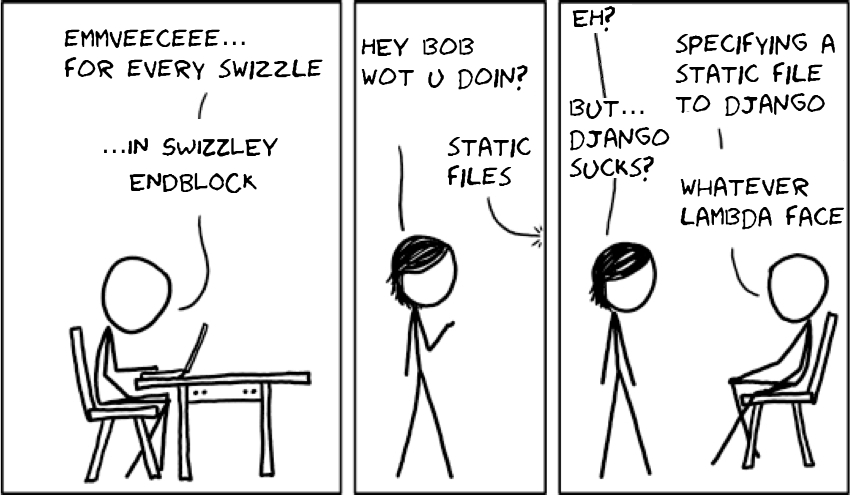
\includegraphics[width=0.7\paperwidth]{image/why-django-sucks.png}
\end{block}
\end{frame}


\begin{frame}
\frametitle{Goals}
\framesubtitle{Our goals for today}
\begin{block}{I could talk all day about why django sucks}
\begin{itemize}
\item<1> and I'd be saying lots and lots of true things
\item<2> but not necessarily helpful things
\end{itemize}
\end{block}
\end{frame}


\begin{frame}
\frametitle{Goals}
\framesubtitle{Our goals for today}
\begin{block}{The goal today}
To equip you with new tools and perspective, with which to explore the question for yourself.
\end{block}
\end{frame}
\begin{frame}
\frametitle{Goals}
\framesubtitle{Lies}
\begin{block}{Along the way}
We will visit some of the lies you have been told
\end{block}
\end{frame}


\begin{frame}
\frametitle{Goals}
\framesubtitle{Lies}
\begin{block}{Tacitly insidious ones}
"Having to come to grips with Monads just isn't worth it for most people"
\end{block}
\end{frame}


\begin{frame}
\frametitle{Goals}
\framesubtitle{Lies}
\begin{block}{Confusingly insidious ones}
"Imperative vs functional programming vs object-oriented programming"
\end{block}
\end{frame}


\begin{frame}
\frametitle{Goals}
\framesubtitle{Lies}
\begin{block}{Awkward ones}
"The real world is mutable"
\end{block}
\end{frame}


\begin{frame}
\frametitle{Goals}
\framesubtitle{Lies}
\begin{block}{Funny ones}
"Django: The Web framework for perfectionists with deadlines"
\end{block}
\end{frame}

\begin{frame}
\frametitle{Goals}
\begin{block}{Summary}
\begin{itemize}
\item What is functional programming?
\item What does monad mean?
\item Functional imperative programming
\item Parametricity \textemdash types are documentation
\end{itemize}
\end{block}
\end{frame}

{
  \newmdenv[tikzsetting={draw=black,fill=white,fill opacity=0.7, line width=4pt},backgroundcolor=none,leftmargin=0,rightmargin=0,innertopmargin=4pt,skipbelow=\baselineskip,%
  skipabove=\baselineskip]{TitleBoxWhatDoesFunctionalProgrammingMean}

  \usebackgroundtemplate{
\includegraphics[width=1.0\paperwidth]{image/title-background.png}}

  \begin{frame}[plain] 
  \title{What is Functional Programming?}
  
  \vspace{3em}

  \begin{TitleBoxWhatDoesFunctionalProgrammingMean}
    \begin{center}
    {\Large \inserttitle}
    \end{center}
  \end{TitleBoxWhatDoesFunctionalProgrammingMean}

  \end{frame}
}


\begin{frame}
\frametitle{Functional Programming}
\begin{block}{Split the question in two}
\begin{itemize}
\item what does functional programming mean in principle?
\item what are the consequences of this principle?
\end{itemize}
\end{block}
\end{frame}


\begin{frame}
\frametitle{Functional Programming}
\begin{block}{What does functional programming mean?}
\begin{itemize}
\item<1> programming with functions
\item<2> yeah right, but what is a function?
\end{itemize}
\end{block}
\end{frame}


\begin{frame}
\frametitle{Functional Programming}
\begin{block}{A function}
relates every argument to a result \textbf{and does nothing else}
\end{block}
\end{frame}


\begin{frame}
\frametitle{Functional Programming}
\begin{block}{Functions give rise to \emph{referential transparency}}
An expression \lstinline$expr$ is referentially transparent if in all programs \lstinline$p$,
all occurrences of \lstinline$expr$ in \lstinline$p$ can be replaced by the result assigned
to \lstinline$expr$ without causing an observable effect on \lstinline$p$.
\end{block}
\end{frame}


\begin{frame}[fragile]
\frametitle{Functional Programming}
\begin{block}{Functions give rise to \emph{referential transparency}}
\begin{lstlisting}[style=python,mathescape]
def p(): 
  x = `expression`
  proc(x, x)
\end{lstlisting}
\begin{tikzpicture}[remember picture,overlay]
\coordinate (aa) at ($(a1)+(5,5.2)$);
\node[note,draw,callout relative pointer={($(aa)-(7.8,2.2)$)},right] at (aa) {is \lstinline$expression$ referentially transparent?};
\end{tikzpicture}
\end{block}
\end{frame}


\begin{frame}[fragile]
\frametitle{Functional Programming}
\begin{block}{Functions give rise to \emph{referential transparency}}
\begin{lstlisting}[style=python,mathescape]
def p(): 
  # x = expression
  proc(`expression`, `expression`)
\end{lstlisting}
\begin{tikzpicture}[remember picture,overlay]
\coordinate (aa) at ($(a1)+(2,2.0)$);
\node[note,draw,callout relative pointer={($(aa)-(4.4,-3.1)$)},right] at (aa) {has this refactoring affected the program?};
\node[note,draw,callout relative pointer={($(aa)-(1.8,-3.1)$)},right] at (aa) {has this refactoring affected the program?};
\end{tikzpicture}
\end{block}
\end{frame}


\begin{frame}[fragile]
\frametitle{Functional Programming}
\begin{block}{Referential Transparency}
\begin{lstlisting}[style=python,mathescape]
def print2(s, t):
  print(s)
  print(t)

def strpopthen():
  s = 'abcdef'
  x = `s[0]`
  print2(x,x)
\end{lstlisting}
\begin{tikzpicture}[remember picture,overlay]
\coordinate (aa) at ($(a1)+(5,4.2)$);
\node[note,draw,callout relative pointer={($(aa)-(8.1,2.5)$)},right] at (aa) {referentially transparent?};
\end{tikzpicture}
\end{block}
\end{frame}


\begin{frame}[fragile]
\frametitle{Functional Programming}
\begin{block}{Referential Transparency}
\begin{lstlisting}[style=python,mathescape]
def print2(s, t):
  print(s)
  print(t)

def strpopthen():
  s = 'abcdef'
  # x = s[0]
  print2(`s[0]`,`s[0]`)
\end{lstlisting}
\begin{tikzpicture}[remember picture,overlay]
\coordinate (aa) at ($(a1)+(1,1.5)$);
\node[note,draw,callout relative pointer={($(aa)-(1.3,-1.9)$)},right] at (aa) {program changed?};
\node[note,draw,callout relative pointer={($(aa)-(0.3,-1.9)$)},right] at (aa) {program changed?};
\end{tikzpicture}
\end{block}
\end{frame}


\begin{frame}[fragile]
\frametitle{Functional Programming}
\begin{block}{Referential Transparency}
\begin{lstlisting}[style=python,mathescape]
def print2(s, t):
  print(s)
  print(t)

def listpopthen():
  s = ['a','b','c','d','e','f']
  x = `s.pop()`
  print2(x,x)
\end{lstlisting}
\begin{tikzpicture}[remember picture,overlay]
\coordinate (aa) at ($(a1)+(5,2.8)$);
\node[note,draw,callout relative pointer={($(aa)-(7.7,0.1)$)},right] at (aa) {referentially transparent?};
\end{tikzpicture}
\end{block}
\end{frame}


\begin{frame}[fragile]
\frametitle{Functional Programming}
\begin{block}{Referential Transparency}
\begin{lstlisting}[style=python,mathescape]
def print2(s, t):
  print(s)
  print(t)

def listpopthen():
  s = ['a','b','c','d','e','f']
  # x = s.pop()
  print2(`s.pop()`,`s.pop()`)
\end{lstlisting}
\begin{tikzpicture}[remember picture,overlay]
\coordinate (aa) at ($(a1)+(1,1.5)$);
\node[note,draw,callout relative pointer={($(aa)-(1.3,-1.8)$)},right] at (aa) {program changed?};
\node[note,draw,callout relative pointer={($(aa)-(-0.3,-1.8)$)},right] at (aa) {program changed?};
\end{tikzpicture}
\end{block}
\end{frame}


\begin{frame}
\frametitle{Functional Programming}
\framesubtitle{What does functional programming mean?}
\begin{block}{The essence of functional programming}
is the demand that expressions, \textbf{in general}, maintain referential transparency
\end{block}
\end{frame}


\begin{frame}
\frametitle{Functional Programming}
\framesubtitle{but why?}
\begin{block}{referential transparency gives rise to, \textbf{and monopolises}}
\begin{itemize}
\item \emph{equational reasoning}

      an essential tool for code readability
\item \emph{modularity}

      delineating concepts, building new programs from slightly smaller programs
\end{itemize}
\end{block}
\end{frame}


\begin{frame}
\frametitle{Functional Programming}
\framesubtitle{therefore}
\begin{block}{Functional Programming is}
\begin{itemize}
\item<1> a thesis, independent of any programming language
\item<2> to some extent, a programming language may provide the programmer assistance in achieving adherence to the thesis
\item<3> not anything more than this, despite what you may have been told
\end{itemize}
\end{block}
\end{frame}


\begin{frame}
\frametitle{Functional Programming}
\framesubtitle{python}
\begin{block}{Well that raises an interesting question}
Does python assist in achieving this objective?
\end{block}
\end{frame}


\begin{frame}
\frametitle{Functional Programming}
\framesubtitle{python}
\begin{center}
\huge{No.}
\end{center}
\normalsize
\end{frame}


\begin{frame}
\frametitle{Functional Programming}
\begin{block}{This question has been explored and answered}
If anyone tells you that python supports functional programming to any (non-trivial) extent, \textbf{they are outright lying to you}
\end{block}
\tiny{and I have the code to prove it}
\end{frame}


\begin{frame}
\frametitle{Functional Programming}
\begin{block}{As a consequence}
Python demands that you, the programmer, forgo many of the most essential tools of progressive software development
\end{block}
\end{frame}

{
  \newmdenv[tikzsetting={draw=black,fill=white,fill opacity=0.7, line width=4pt},backgroundcolor=none,leftmargin=0,rightmargin=0,innertopmargin=4pt,skipbelow=\baselineskip,%
  skipabove=\baselineskip]{TitleBoxWhatDoesMonadMean}

  \usebackgroundtemplate{
\includegraphics[width=1.0\paperwidth]{image/title-background.png}}

  \begin{frame}[plain] 
  \title{What Does Monad Mean?}
  
  \vspace{3em}

  \begin{TitleBoxWhatDoesMonadMean}
    \begin{center}
    {\Large \inserttitle}
    \end{center}
  \end{TitleBoxWhatDoesMonadMean}

  \end{frame}
}


\begin{frame}
\frametitle{What Does Monad Mean?}
\begin{block}{Well if you google it}
burritos, spacesuits or some shit like that
\end{block}
% wrong question
\end{frame}


\begin{frame}
\frametitle{What Does Monad Mean?}
\begin{block}{I want to do three things}
\begin{enumerate}
  \item establish the principles of abstraction and what is required to exploit them
  \item come to understand the relationship between monads and functional programming \emph{\tiny{(spoiler: there isn't one)}} \normalsize
  \item arm you with the skills to recognise common myths
\end{enumerate}
\end{block}
\end{frame}


\begin{frame}
\frametitle{Principles and Goals of Abstraction}
\begin{block}{Construct a constraint}
\begin{itemize}
  \item minimise the requirements to satisfy the constraint to increase instances
  \item maximise potential for deriving operations as a consequence of satisfying the constraint 
\end{itemize}
\end{block}
\end{frame}


\begin{frame}
\frametitle{Principles and Goals of Abstraction}
\begin{block}{Trade-off between the two}
\begin{itemize}
  \item stronger constraint
    \begin{itemize}
      \item fewer instances
      \item more derived operations
    \end{itemize}
  \item weaker constraint
    \begin{itemize}
      \item more instances
      \item fewer derived operations
    \end{itemize}
\end{itemize}
\end{block}
\end{frame}


\begin{frame}
\frametitle{Principles and Goals of Abstraction}
\begin{block}{The ultimate goal}
Avoid repetition of the same work
\end{block}
\end{frame}


\begin{frame}
\frametitle{Principles and Goals of Abstraction}
\begin{block}{Consequently}
A proposed abstraction that loses in both directions is a \emph{false economy} and must be efficiently discarded
\end{block}
\end{frame}


\begin{frame}
\frametitle{Monad}
\begin{block}{Monad is another abstraction}
\begin{itemize}
  \item not expressible in degenerate static type systems
  \item difficult to demonstrate without a static type system
\end{itemize}
\end{block}
\end{frame}


\begin{frame}[fragile]
\frametitle{Monad}
\begin{block}{So sorry, but I must use a practical programming language now}
\begin{lstlisting}[style=haskell,mathescape]
class Monad f where
  (=<<) :: (a -> f b) -> f a -> f b
  unit  :: x -> f x
\end{lstlisting}
\end{block}
\end{frame}


\begin{frame}[fragile]
\frametitle{Monad}
\begin{block}{This abstraction has many instances (values for \lstinline$f$)}
\begin{itemize}
  \item list
  \item continuations
  \item nullable values
  \item exception chaining
  \item state
  \item I/O actions
  \item argument threading
  \item logging
  \item \emph{hundreds more}
\end{itemize}
\end{block}
\end{frame}


\begin{frame}
\frametitle{Monad}
\begin{block}{This abstraction gives rise to many useful operations}
\begin{itemize}
  \item sequencing a list of effect values

        \lstinline$[f a] -> f [a]$
  \item replicating an effect a given number of times

        \lstinline$Int -> f a -> f [a]$
  \item \emph{bazillions more}
\end{itemize}
\end{block}
\end{frame}


\begin{frame}
\frametitle{Monad}
\begin{block}{We just saw}
\begin{itemize}
  \item<1> the monad abstraction expressed as a constraint
  \item<2> instances that satisfy the constraint
  \item<3> operations that are derived from the constraint
  \item<4> \textbf{Do not conflate these}
\end{itemize}
\end{block}
\end{frame}


\begin{frame}
\frametitle{Abstraction nomenclature}
\begin{block}{Other abstractions trade off along the two competing principles}
\begin{itemize}
  \item covariant functor
  \item applicative functor
  \item semigroupoid
  \item comonad
  \item profunctor
  \item monoid
  \item \emph{hundreds more}
\end{itemize}
\end{block}
\end{frame}


\begin{frame}
\frametitle{Now that we know this}
\begin{block}{We can do some mythbusting}
\begin{itemize}
  \item<1-> Monads are for side-effects
  \item<2-> Monads are for functional programming only
  \item<3-> Monads are for doing I/O
  \item<4-> Monads don't apply to my programming tasks
  \item<5-> I use Python, so monads won't help me as much
\end{itemize}
\visible<6->{
  \begin{tikzpicture}[remember picture,overlay]
  \coordinate (aa) at ($(a1)+(1,4.5)$);
  \node[right] at (aa) {
\includegraphics[height=3cm]{image/bullshizzles.png}};
  \end{tikzpicture}
}
\end{block}
\end{frame}


\begin{frame}
\frametitle{Bullshizzles}
\begin{block}{Perfidious Seduction}
You will be invited to believe these things. Decide wisely.
\end{block}
\end{frame}


\begin{frame}
\frametitle{Abstraction and Python}
\begin{block}{Python}
Python achieves abstraction using dynamic structural-typing\footnote{aka duck typing}
\end{block}
\end{frame}


\begin{frame}
\frametitle{Abstraction and Python}
\begin{block}{Further to this}
You will rarely see even the most fundamental abstractions in these systems
\end{block}
\end{frame}


\begin{frame}
\frametitle{Abstraction and Python}
\begin{block}{Certainly}
You will never see any non-trivial abstraction \tiny{\emph{(above those already mentioned)}}\normalsize
\end{block}
\end{frame}


\begin{frame}
\frametitle{Abstraction and Python}
\begin{center}
\huge{Why might this be?}
\end{center}
\normalsize
\end{frame}

{
  \newmdenv[tikzsetting={draw=black,fill=white,fill opacity=0.7, line width=4pt},backgroundcolor=none,leftmargin=0,rightmargin=0,innertopmargin=4pt,skipbelow=\baselineskip,%
  skipabove=\baselineskip]{TitleBoxFunctionalImperativeProgramming}

  \usebackgroundtemplate{
\includegraphics[width=1.0\paperwidth]{image/title-background.png}}

  \begin{frame}[plain] 
  \title{Functional Imperative Programming}
  
  \vspace{3em}

  \begin{TitleBoxFunctionalImperativeProgramming}
    \begin{center}
    {\Large \inserttitle}
    \end{center}
  \end{TitleBoxFunctionalImperativeProgramming}

  \end{frame}
}


\begin{frame}
\frametitle{Functional v Imperative v OOP}
\framesubtitle{The fallacy of false compromise}
\begin{block}{A note on OOP}
I am going to dismiss Object-Oriented Programming, because I don't know what it is \tiny{and neither do you}
\end{block}
\end{frame}


{
\usebackgroundtemplate{
\includegraphics[width=1.0\paperwidth]{image/book.png}}
\begin{frame}
\frametitle{Functional v Imperative}
\begin{center}
\LARGE{The parable of he who is not even wrong}
\end{center}
\end{frame}
}

{
\usebackgroundtemplate{
\begin{tikzpicture}[remember picture,overlay]
  \coordinate (aa) at ($(a1)+(-1,7.5)$);
  \node[right] at (aa) {
\includegraphics[height=1cm]{image/book-small.png}};
\end{tikzpicture}
}

\begin{frame}
\frametitle{Functional v Imperative}
\framesubtitle{The parable of he who is not even wrong}
Someone in a pub once said to me, not too long ago
\begin{quote}
Hi my name is Wiggleydoo and I am the Chief Python Wippedy-wop for Hoopdiddy-zip
\end{quote}
\end{frame}


\begin{frame}
\frametitle{Functional v Imperative}
\framesubtitle{The parable of he who is not even wrong}
and I thought to myself, ``oh yeah that's nice''
\end{frame}


\begin{frame}
\frametitle{Functional v Imperative}
\framesubtitle{The parable of he who is not even wrong}
and then this happened
\begin{quote}
Functional programming is great and all, but I only use state where it is appropriate. You know\ldots when the problem demands stateful things.
\end{quote}
\end{frame}


\begin{frame}
\frametitle{Functional v Imperative}
\framesubtitle{The parable of he who is not even wrong}
\begin{center}
and it all came back to me
\end{center}
\begin{center}

\includegraphics[width=0.7\paperwidth]{image/shock.jpg}
\end{center}
\end{frame}


\begin{frame}
\frametitle{Functional v Imperative}
\framesubtitle{The parable of he who is not even wrong}
\begin{block}{Fact}
There is no such thing as an ``inherently stateful'' computation or algorithm
\end{block}
\end{frame}


\begin{frame}
\frametitle{Functional v Imperative}
\framesubtitle{The parable of he who is not even wrong}
\begin{block}{So I called shenanigans on that}
\begin{quote}
but what about those algorithms that demand imperative programming?
\end{quote}
\end{block}
\end{frame}


\begin{frame}
\frametitle{Functional v Imperative}
\framesubtitle{The parable of he who is not even wrong}
\begin{block}{Church-Turing Thesis}
\begin{quote}
Many people do imperative programming using pure-functional programming all day, every day
\end{quote}
This can be achieved for every program that can possibly exist
\end{block}
\end{frame}


\begin{frame}
\frametitle{Functional v Imperative}
\framesubtitle{The parable of he who is not even wrong}
\begin{block}{``but how?''}
At this point I am stumped. ``Casually \ldots er neatly?''
\end{block}
\end{frame}


\begin{frame}
\frametitle{Functional v Imperative}
\framesubtitle{The parable of he who is not even wrong}
\begin{block}{Recognising my confoundment}
My friend pulled out some imperative pure-functional production code that had been written at a bank
\end{block}
\end{frame}


\begin{frame}
\frametitle{Functional v Imperative}
\framesubtitle{The parable of he who is not even wrong}
\begin{block}{Escaping the state of delirium}
The discussion then quickly turned to beer
\end{block}
\end{frame}
}


\begin{frame}[fragile]
\frametitle{Functional v Imperative}
\begin{block}{Here is an imperative Haskell program}
\begin{lstlisting}[style=haskell,mathescape]
program = do
  a <- readFile "file"
  print a
  writeFile "cods!" "file"
  b <- readFile "file"
  print b
\end{lstlisting}
\end{block}
\end{frame}


\begin{frame}[fragile]
\frametitle{Functional v Imperative}
\begin{block}{Here is an imperative Haskell program}
\begin{lstlisting}[style=haskell,mathescape]
program = do
  a <- `readFile "file"`
  print a
  writeFile "cods!" "file"
  b <- `readFile "file"`
  print b
\end{lstlisting}
\end{block}
\begin{tikzpicture}[remember picture,overlay]
\coordinate (aa) at ($(a1)+(5,5.8)$);
\node[note,draw,callout relative pointer={($(aa)-(5.7,4.0)$)},right] at (aa) {well?};
\node[note,draw,callout relative pointer={($(aa)-(5.9,5.1)$)},right] at (aa) {well?};
\end{tikzpicture}
\end{frame}


\begin{frame}[fragile]
\frametitle{Functional v Imperative}
\begin{block}{Here is an imperative Haskell program}
\begin{lstlisting}[style=haskell,mathescape]
file =
  readFile "file"

program = do
  a <- `file`
  print a
  writeFile "cods!" "file"
  b <- `file`
  print b
\end{lstlisting}
\end{block}
\begin{tikzpicture}[remember picture,overlay]
\coordinate (aa) at ($(a1)+(5,4.2)$);
\node[note,draw,callout relative pointer={($(aa)-(7.8,2.4)$)},right] at (aa) {did the program change?};
\node[note,draw,callout relative pointer={($(aa)-(8.3,3.2)$)},right] at (aa) {did the program change?};
\end{tikzpicture}
\end{frame}


\begin{frame}[fragile]
\frametitle{Functional v Imperative}
\begin{block}{Here is an imperative Haskell program}
\begin{lstlisting}[style=haskell,mathescape]
file =
  readFile "file"

program = do
  `a <- file`
  `print a`
  writeFile "cods!" "file"
  `b <- file`
  `print b`
\end{lstlisting}
\end{block}
\begin{tikzpicture}[remember picture,overlay]
\coordinate (aa) at ($(a1)+(5,4.2)$);
\node[note,draw,callout relative pointer={($(aa)-(8.0,2.6)$)},right] at (aa) {in fact, look at this repetition of work};
\node[note,draw,callout relative pointer={($(aa)-(9.8,3.7)$)},right] at (aa) {in fact, look at this repetition of work};
\end{tikzpicture}
\end{frame}


\begin{frame}[fragile]
\frametitle{Functional v Imperative}
\begin{block}{Here is an imperative Haskell program}
\begin{lstlisting}[style=haskell,mathescape]
printfile = do
  f <- readFile "file"
  print f

program = do
  `printfile`
  writeFile "cods!" "file"
  `printfile`
\end{lstlisting}
\end{block}
\end{frame}


\begin{frame}[fragile]
\frametitle{Functional v Imperative}
\begin{block}{Did I mention that functional programming is}
\begin{center}
\textbf{Don't Repeat Yourself} without the duplicity?
\end{center}
\end{block}
\end{frame}


\begin{frame}[fragile]
\frametitle{Functional v Imperative}
\begin{block}{Here is an imperative Haskell program}
\begin{lstlisting}[style=haskell,mathescape]
printfile = do
  f <- readFile "file"
  print f

program = do
  `printfile`
  writeFile "cods!" "file"
  `printfile`
\end{lstlisting}
\end{block}
\begin{tikzpicture}[remember picture,overlay]
\coordinate (aa) at ($(a1)+(7,4.2)$);
\node[note,draw,callout relative pointer={($(aa)-(11.8,2.6)$)},right] at (aa) {stop it!};
\node[note,draw,callout relative pointer={($(aa)-(11.8,3.3)$)},right] at (aa) {stop it!};
\end{tikzpicture}
\end{frame}


\begin{frame}[fragile]
\frametitle{Functional v Imperative}
\begin{block}{Here is an imperative Haskell program}
\begin{lstlisting}[style=haskell,mathescape]
a >.> b = do
  a
  b
  a
  
printfile = do
  f <- readFile "file"
  print f

program =
  printfile >.> writeFile "cods!" "file"
\end{lstlisting}
\end{block}
\end{frame}


\begin{frame}[fragile]
\frametitle{Functional v Imperative}
\begin{block}{We can do this equational reasoning on imperative programs}
\textbf{because we are functional programming}
\end{block}
\end{frame}


\begin{frame}[fragile]
\frametitle{Functional v Imperative}
\begin{itemize}
  \item<1-> Functional Programming
  \item<2-> or Imperative Programming
  \item<3-> \textbf{but never both}
\end{itemize}
\visible<4->{
  \begin{tikzpicture}[remember picture,overlay]
  \coordinate (aa) at ($(a1)+(0,4.7)$);
  \node[right] at (aa) {
\includegraphics[height=3cm]{image/bullshizzles.png}};
  \end{tikzpicture}
}
\end{frame}


\begin{frame}[fragile]
\frametitle{Functional v Imperative}
\begin{block}{Functional programming is}
just a \tiny{not ridiculous}\normalsize{ means of imperative programming}
\end{block}
\end{frame}


\begin{frame}[fragile]
\frametitle{Functional v Imperative}
\begin{block}{To further help demonstrate this point}
\begin{itemize}
  \item<1> pure-functional random value library using the C\# programming language
  \item<2> pure-functional RDBMS library using the Java programming language
  \item<3> pure-functional terminal I/O programs using the Ruby programming language
\end{itemize}
\end{block}
\end{frame}


\begin{frame}[fragile]
\frametitle{Functional v Imperative}
``I don't think the benefits of enforcing side-effect-free code (even optionally) make up for the many work-arounds you have to use to get anything done in the real world.''
\begin{center}

\includegraphics[width=0.1\paperwidth]{image/lalala.png}
\end{center}
``[Functional Programming makes] the code pretty unreadable for people who aren't used to functional''
\end{frame}

% 

{
  \newmdenv[tikzsetting={draw=black,fill=white,fill opacity=0.7, line width=4pt},backgroundcolor=none,leftmargin=0,rightmargin=0,innertopmargin=4pt,skipbelow=\baselineskip,%
  skipabove=\baselineskip]{TitleBoxParametricity}

  \usebackgroundtemplate{
\includegraphics[width=1.0\paperwidth]{image/title-background.png}}

  \begin{frame}[plain] 
  \title{Parametricity}
  \subtitle{types are documentation}
  
  \vspace{3em}

  \begin{TitleBoxParametricity}
    \begin{center}
    {\Large \inserttitle}
    \end{center}
  \end{TitleBoxParametricity}

  \end{frame}
}


\begin{frame}
\frametitle{Parametricity}
\begin{block}{Parametricity, or Theorems for Free, is}
a technique described by Wadler\cite{wadler1989theorems} that gives rise to many practical consequences.
\end{block}
\end{frame}


\begin{frame}
\frametitle{Parametricity}
\begin{block}{One practical consequence of parametricity is that}
Types, by exploiting generalisation, may be utilised to document code and that documentation never goes out of date.
\end{block}
\end{frame}


\begin{frame}
\frametitle{Parametricity}
\begin{center}
Many nutty things have been said about static typing \ldots
\end{center}
\begin{center}

\includegraphics[width=0.5\paperwidth]{image/static-typing-nutty.png}
\end{center}
\end{frame}

{
\usebackgroundtemplate{
\begin{tikzpicture}[remember picture,overlay]
  \coordinate (aa) at ($(a1)+(-1,7.5)$);
  \node[right] at (aa) {
\includegraphics[height=1cm]{image/book-small.png}};
\end{tikzpicture}
}

\begin{frame}
\frametitle{Parametricity}
\begin{block}{\ldots including this one time}
a neurotic colleague insisted that static typing is terrible \ldots
\end{block}
\end{frame}


\begin{frame}[fragile]
\frametitle{Parametricity}
\ldots because you have to write messy types all the time!
\begin{lstlisting}[style=python,mathescape]
`int x`
x = 3
`String y`
y = "abc"
`(String, Int) a`
a = ("xyz", 9)
`[Int] b`
b = [1,4,9,16,x]
\end{lstlisting}
\end{frame}


\begin{frame}[fragile]
\frametitle{Parametricity}
So I took the Python source file
\begin{lstlisting}[style=python,mathescape]
x = 3
y = "abc"
a = ("xyz", 9)
b = [1,4,9,16,x]
\end{lstlisting}
\end{frame}


\begin{frame}[fragile]
\frametitle{Parametricity}
\ldots and loaded it into the Glasgow Haskell Compiler repl
\begin{lstlisting}
> ln -s soneat.py notypes.hs
> ghci notypes.hs
\end{lstlisting}
\end{frame}

}


\begin{frame}
\frametitle{Parametricity}
\begin{block}{The goal is to tell you about}
a more subtle, and rarely discussed, advantage that is available by appropriately exploiting types
\end{block}
\tiny{not so much to engage the static typing debate itself}
\end{frame}


\begin{frame}
\frametitle{Parametricity}
\framesubtitle{Theorems for Free!}
\begin{block}{Philip Wadler \cite{wadler1989theorems} tells us:}
\begin{quotation}
Write down the definition of a polymorphic function on a piece of paper. Tell me its type, but be careful not to let me see the function's definition. I will tell you a theorem that the function satisfies.

The purpose of this paper is to explain the trick.
\end{quotation}
\end{block}
\end{frame}


\begin{frame}
\frametitle{Totality}
\framesubtitle{Fast and loose reasoning is morally correct}
\begin{block}{Danielsson, Hughes, Jansson \& Gibbons \cite{danielsson2006fast} tell us:}
\begin{quotation}
Functional programmers often reason about programs as if
they were written in a total language, expecting the results
to carry over to non-total (partial) languages. We justify
such reasoning.
\end{quotation}
\end{block}
\end{frame}


\begin{frame}[fragile]
\frametitle{Parametricity}
\begin{block}{What if I told you}
\begin{quotation}
There exists a function that takes a list of some element type and returns a list of elements of that same type? 
\end{quotation}
\begin{lstlisting}[style=haskell]
function :: [a] -> [a]
\end{lstlisting}
\end{block}
\end{frame}


\begin{frame}[fragile]
\frametitle{Parametricity}
\begin{block}{I observe that}
there is nothing else to know about this element type
\end{block}
Its declared structure is \emph{universally quantified}
\end{frame}


\begin{frame}
\frametitle{Parametricity}
\begin{block}{On this information alone, I can $\therefore$ conclude that}
\textbf{Theorem:} every element in the result appears in the input
\end{block}
\end{frame}


\begin{frame}
\frametitle{Parametricity}
\framesubtitle{Fast and Loose Reasoning}
\begin{block}{Morally Correct?}
What does it mean to ``reason as if we were in a total language, expecting the results to carry over to non-total languages''?
\end{block}
\end{frame}


\begin{frame}
\frametitle{Parametricity}
\framesubtitle{Fast and Loose Reasoning}
\begin{block}{It means we can ``morally'' exclude logical-inconsistencies $\bot$}
\begin{itemize}
  \item Type-case (e.g. \lstinline{is})
  \item Type-cast
  \item Type-value (e.g. \lstinline{type})
  \item unsafe universal functions e.g. \lstinline{str}, \lstinline{int}
  \item side-effects
  \item \lstinline{None} or \lstinline{null}
  \item exceptions
  \item Infinite recursion
\end{itemize}
\end{block}
\end{frame}


\begin{frame}
\frametitle{Parametricity}
\framesubtitle{Fast and Loose Reasoning}
\begin{block}{Some non-total systems do not have these $\bot$ values anyway}
\begin{itemize}
  \item \sout{Type-case e.g. (\lstinline{is})}
  \item \sout{Type-cast}
  \item \sout{Type-value e.g. (\lstinline{type})}
  \item \sout{unsafe universal functions e.g. \lstinline{str}, \lstinline{int}}
  \item \sout{side-effects}
  \item \sout{\lstinline{None} or \lstinline{null}}
  \item exceptions
  \item Infinite recursion
\end{itemize}
\end{block}
\end{frame}


\begin{frame}[fragile]
\frametitle{Parametricity}
\framesubtitle{Fast and Loose Reasoning}
\begin{block}{On the basis of fast and loose reasoning}
Can we invalidate the theorem, \textbf{every element in the result appears in the input}?
\end{block}
\begin{lstlisting}[style=haskell]
function :: [a] -> [a]
\end{lstlisting}
\end{frame}


\begin{frame}
\frametitle{Parametricity}
\begin{block}{OK, so we have machine-checked documentation, but}
How do we know what this function does exactly?
\end{block}
\end{frame}


\begin{frame}
\frametitle{Parametricity}
\begin{block}{We can write unit tests}
but not your laborious and clumsy kind
\end{block}
\end{frame}


\begin{frame}[fragile]
\frametitle{Parametricity}
\begin{block}{Specification-based tests or universally quantified properties\cite{claessen2011quickcheck}}
\begin{itemize}
  \item<1-> \lstinline[style=haskell,mathescape]{$\forall$ x. function [x] == [x]}
  \item<1-> \lstinline[style=haskell,mathescape]{$\forall$ x y. function (x ++ y) == function y ++ function x}
  \item<2-> Reminder: \lstinline{function :: [a] -> [a]}
  \item<2-> Now what does our \lstinline{function} do?
\end{itemize}
\end{block}
\end{frame}


\begin{frame}[fragile]
\frametitle{Parametricity}
\begin{block}{More theorems for free}
\begin{itemize}
  \item<1-> comp :: (a -> b) -> (b -> c) -> (a -> c)
  \item<2-> choose :: (a, a) -> a
\end{itemize}
\begin{lstlisting}
\end{lstlisting}
\end{block}
\end{frame}

{
  \newmdenv[tikzsetting={draw=black,fill=white,fill opacity=0.7, line width=4pt},backgroundcolor=none,leftmargin=0,rightmargin=0,innertopmargin=4pt,skipbelow=\baselineskip,%
  skipabove=\baselineskip]{TitleBoxBravery}

  \usebackgroundtemplate{
\includegraphics[width=1.0\paperwidth]{image/title-background.png}}

  \begin{frame}[plain] 
  \title{A note on your bravery}
  
  \vspace{3em}

  \begin{TitleBoxBravery}
    \begin{center}
    {\Large \inserttitle}
    \end{center}
  \end{TitleBoxBravery}

  \end{frame}
}


\begin{frame}
\frametitle{Introspection}
\begin{block}{So}
I typed ``functional programming for python'' into an internet search \ldots
\end{block}
\end{frame}


{
\usebackgroundtemplate{
\begin{tikzpicture}[remember picture,overlay]
  \coordinate (aa) at ($(a1)+(0,7.5)$);
  \node[right] at (aa) {
\includegraphics[height=1cm]{image/punch.jpg}};
\end{tikzpicture}
}


\begin{frame}
\frametitle{Bravery}
\begin{block}{Functional Programming \ldots}
The designers [of functional programming languages] \ldots choose to emphasize one particular approach to programming
\includegraphics[height=0.4cm]{image/bullshit.jpg} This is \ldots difficult to write programs that use a different approach
\includegraphics[height=0.4cm]{image/bullshit.jpg} Other languages are multi-paradigm languages that support several different approaches. Lisp, C++, and Python are multi-paradigm \ldots can write programs \ldots procedural, object-oriented, or functional in all of these languages
\includegraphics[height=0.4cm]{image/bullshit.jpg}
\end{block}
\end{frame}


\begin{frame}
\frametitle{Bravery}
\begin{block}{Some languages \ldots}
Some [functional programming] languages don't even have assignment statements such as \lstinline$a=3$ or \lstinline{c=a+b}
\includegraphics[height=0.4cm]{image/bullshit.jpg}, but it's difficult to avoid all side effects
\includegraphics[height=0.4cm]{image/bullshit.jpg} Printing to the screen or writing to a disk file are side effects, for example
\includegraphics[height=0.4cm]{image/bullshit.jpg}
\end{block}
\end{frame}


\begin{frame}
\frametitle{Bravery}
\begin{block}{Formal provability}
A theoretical benefit is that it’s easier to construct a mathematical proof that a functional program is correct
\includegraphics[height=0.4cm]{image/bullshit.jpg} \ldots Unfortunately, proving programs correct is largely impractical
\includegraphics[height=0.4cm]{image/bullshit.jpg} and not relevant to Python software
\includegraphics[height=0.4cm]{image/bullshit.jpg}
\end{block}
\end{frame}


\begin{frame}
\frametitle{Bravery}
\begin{block}{iterators}
a Python language feature that's an important foundation for writing functional-style programs: \textbf{iterators}
\includegraphics[height=0.4cm]{image/bullshit.jpg}
\end{block}
\end{frame}

}

{
\usebackgroundtemplate{
\begin{tikzpicture}[remember picture,overlay]
  \coordinate (aa) at ($(a1)+(0,7.5)$);
  \node[right] at (aa) {
\includegraphics[height=2cm]{image/brave.jpg}};
\end{tikzpicture}
}

\begin{frame}
\frametitle{Introspection}
\begin{block}{Just when}
Just when I thought I'd seen enough, I realised \textbf{just how brave you all are}
\end{block}
\end{frame}

}
{
  \newmdenv[tikzsetting={draw=black,fill=white,fill opacity=0.7, line width=4pt},backgroundcolor=none,leftmargin=0,rightmargin=0,innertopmargin=4pt,skipbelow=\baselineskip,%
  skipabove=\baselineskip]{TitleBoxConclusion}

  \usebackgroundtemplate{
\includegraphics[width=1.0\paperwidth]{image/title-background.png}}

  \begin{frame}[plain] 
  \title{Let's tie it up}
  
  \vspace{3em}

  \begin{TitleBoxConclusion}
    \begin{center}
    {\Large \inserttitle}
    \end{center}
  \end{TitleBoxConclusion}

  \end{frame}
}


\begin{frame}
\frametitle{Django}
\begin{center}
The primary purpose of frameworks like Django is to observe similarities in otherwise disjoint applications \ldots
\end{center}
\vspace{3em}
\begin{center}

\includegraphics[width=0.4\paperwidth]{image/venn-disjoint.png}
\end{center}
\end{frame}


\begin{frame}
\frametitle{Django}
\begin{center}
\ldots and provide library support for those similarities, while distingushing from differences.
\end{center}
\vspace{3em}
\begin{center}
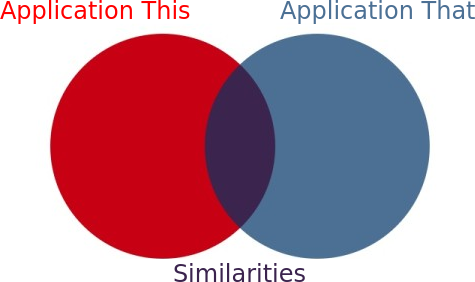
\includegraphics[width=0.4\paperwidth]{image/venn-joined.png}
\end{center}
\end{frame}


\begin{frame}
\frametitle{Django}
\begin{center}
For example, Django \emph{themes} or \emph{templates}
\end{center}
\vspace{3em}
\begin{center}
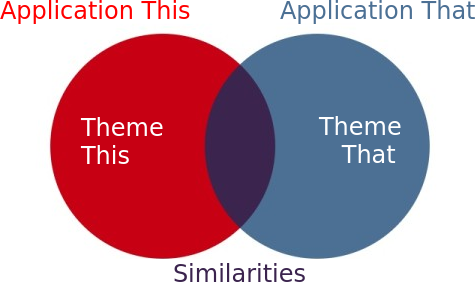
\includegraphics[width=0.4\paperwidth]{image/venn-themes.png}
\end{center}
\end{frame}


\begin{frame}
\frametitle{Bugs}
\begin{block}{Maintenance issues}
Maintenance issues come about when software components leak over these boundaries
\end{block}
\end{frame}


\begin{frame}
\frametitle{Equational Reasoning}
\begin{block}{We have a name for this delineation of concepts}
Equational reasoning
\end{block}
\vspace{3em}
\begin{center}
This is the essence of functional programming!
\end{center}
\end{frame}


\begin{frame}
\frametitle{Tool Support}
OK, so what support do our tools provide us for exploiting this?
\end{frame}


\begin{frame}
\frametitle{Tool Support}
\begin{center}
\huge{0}\normalsize
\end{center}
\vspace{2em}
\begin{center}

\includegraphics[width=0.3\paperwidth]{image/watermelon.png}
\end{center}
\vspace{1em}
\begin{center}
\tiny{``Is it really such a big deal to rewrite your function to use a loop?''}\normalsize
\end{center}
\end{frame}


\begin{frame}
\frametitle{Tool Support}
\begin{center}
Oh
\end{center}
\vspace{2em}
\begin{center}

\includegraphics[width=0.3\paperwidth]{image/sad-face.jpg}
\end{center}
\vspace{1em}
\begin{center}
Then what about parametricity? Abstraction?
\end{center}
\end{frame}


\begin{frame}
\frametitle{Tool Support}
\begin{center}
\huge{Again, 0}\normalsize
\end{center}
\vspace{2em}
\begin{center}

\includegraphics[width=0.3\paperwidth]{image/watermelon.png}
\end{center}
\end{frame}


\begin{frame}
\frametitle{Tool Support}
\begin{block}{More to the point}
There is a \textbf{huge} amount of code that I cannot write without these tools \ldots
\end{block}
\end{frame}


\begin{frame}
\frametitle{Tool Support}
\begin{block}{\ldots and I suspect}
that nobody can, because I never see it
\end{block}
\end{frame}


\begin{frame}
\frametitle{So here's why}
\begin{block}{If you accept}
\begin{itemize}
  \item Equational reasoning
  \item Parametricity
  \item Abstraction
\end{itemize}
\end{block}
\end{frame}


\begin{frame}
\frametitle{So here's why}
\begin{block}{Then you also accept}
\begin{center}

\includegraphics[width=0.3\paperwidth]{image/watermelon.png}
\end{center}
\end{block}
\end{frame}


\begin{frame}
\frametitle{How?}
\begin{block}{How might I learn to exploit these tools?}
\begin{center}
\huge{Diversify}\normalsize
\end{center}
\begin{itemize}
  \item Total programming (Agda, Coq, Idris)
  \item Pure functional programming (Haskell)
\end{itemize}
\end{block}
\end{frame}


\begin{frame}
\frametitle{TL;DR}
\begin{block}{TL;DR}
\begin{center}

\includegraphics[width=0.85\paperwidth]{image/pythonic.png}
\end{center}
\end{block}
\end{frame}

\begin{frame}
\frametitle{References}

\bibliographystyle{amsalpha}
\bibliography{djangocon-2014}
% Church-Turing Thesis
% Cardelli, A Theory of Objects

\end{frame}

\begin{frame}
\frametitle{Licence Attributions}
\begin{itemize}
\item Some images used in this presentation are attributed to Joshua Morris
\item Some images used in this presentation are attributed to XKCD released under the CC BY-NC licence
\item Some images used in this presentation are attributed to NatSilva released under the CC BY-NC-ND licence
\item Some ideas in BeamerTitleSlide by Daniel Falster are used in this presentation
\end{itemize}
\end{frame}


\end{document}
